\documentclass{standalone}
\usepackage{tikz}
\usetikzlibrary{patterns, positioning}


\begin{document}
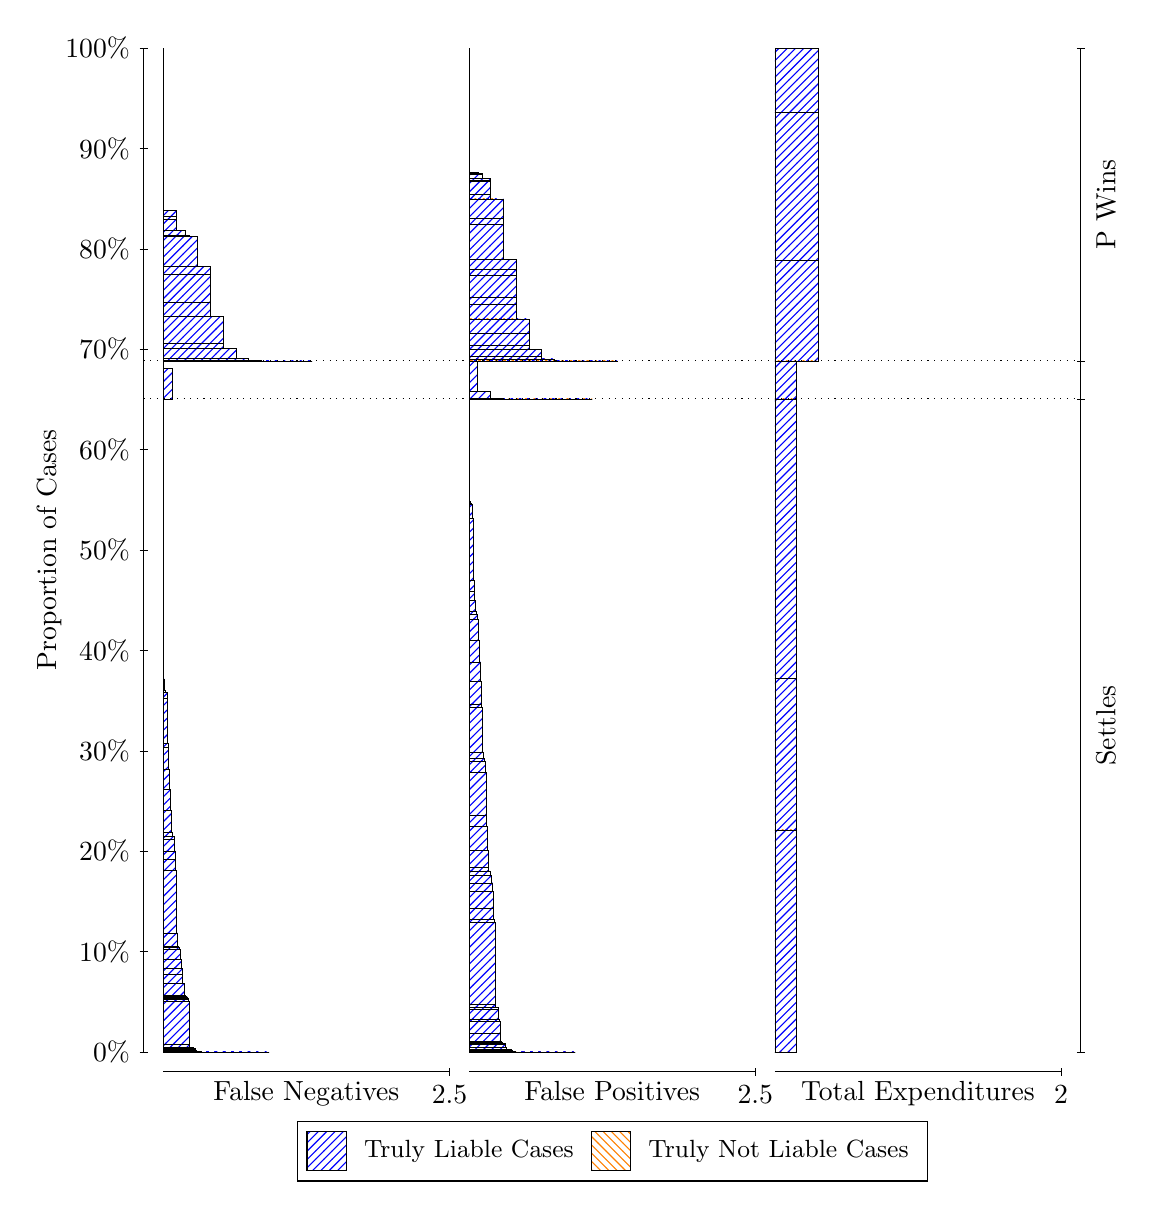
\begin{tikzpicture}
\draw[black, very thin] (1.5,1.75) -- (1.5,14.5);
\node[rotate=90, text=black, anchor=center] at (0.3, 8.125) {Proportion of Cases};
\draw[black, very thin] (1.45,1.75) -- (1.55,1.75);
\node[text=black, anchor=east] at (1.45, 1.75) {0\%};
\draw[black, very thin] (1.45,3.025) -- (1.55,3.025);
\node[text=black, anchor=east] at (1.45, 3.025) {10\%};
\draw[black, very thin] (1.45,4.3) -- (1.55,4.3);
\node[text=black, anchor=east] at (1.45, 4.3) {20\%};
\draw[black, very thin] (1.45,5.575) -- (1.55,5.575);
\node[text=black, anchor=east] at (1.45, 5.575) {30\%};
\draw[black, very thin] (1.45,6.85) -- (1.55,6.85);
\node[text=black, anchor=east] at (1.45, 6.85) {40\%};
\draw[black, very thin] (1.45,8.125) -- (1.55,8.125);
\node[text=black, anchor=east] at (1.45, 8.125) {50\%};
\draw[black, very thin] (1.45,9.4) -- (1.55,9.4);
\node[text=black, anchor=east] at (1.45, 9.4) {60\%};
\draw[black, very thin] (1.45,10.675) -- (1.55,10.675);
\node[text=black, anchor=east] at (1.45, 10.675) {70\%};
\draw[black, very thin] (1.45,11.95) -- (1.55,11.95);
\node[text=black, anchor=east] at (1.45, 11.95) {80\%};
\draw[black, very thin] (1.45,13.225) -- (1.55,13.225);
\node[text=black, anchor=east] at (1.45, 13.225) {90\%};
\draw[black, very thin] (1.45,14.5) -- (1.55,14.5);
\node[text=black, anchor=east] at (1.45, 14.5) {100\%};

\draw[black, very thin] (13.4,1.75) -- (13.4,14.5);
\draw[black, very thin] (13.35,1.75) -- (13.45,1.75);
\node[anchor=west] at (13.35, 1.75) {};
\draw[black, very thin] (13.35,10.044) -- (13.45,10.044);
\node[anchor=west] at (13.35, 10.044) {};
\draw[black, very thin] (13.35,10.526) -- (13.45,10.526);
\node[anchor=west] at (13.35, 10.526) {};
\draw[black, very thin] (13.35,14.5) -- (13.45,14.5);
\node[anchor=west] at (13.35, 14.5) {};

\draw[black, very thin, pattern color=blue, pattern=north east lines] (1.75,1.75) rectangle (3.0943,1.75);
\draw[black, very thin, pattern color=blue, pattern=north east lines] (1.75,1.75) rectangle (3.0217,1.75);
\draw[black, very thin, pattern color=blue, pattern=north east lines] (1.75,1.75) rectangle (2.949,1.75);
\draw[black, very thin, pattern color=blue, pattern=north east lines] (1.75,1.75) rectangle (2.9329,1.75);
\draw[black, very thin, pattern color=blue, pattern=north east lines] (1.75,1.75) rectangle (2.8763,1.75);
\draw[black, very thin, pattern color=blue, pattern=north east lines] (1.75,1.75) rectangle (2.8602,1.75);
\draw[black, very thin, pattern color=blue, pattern=north east lines] (1.75,1.75) rectangle (2.8037,1.75);
\draw[black, very thin, pattern color=blue, pattern=north east lines] (1.75,1.75) rectangle (2.7875,1.75);
\draw[black, very thin, pattern color=blue, pattern=north east lines] (1.75,1.75) rectangle (2.7714,1.75);
\draw[black, very thin, pattern color=blue, pattern=north east lines] (1.75,1.75) rectangle (2.731,1.75);
\draw[black, very thin, pattern color=blue, pattern=north east lines] (1.75,1.75) rectangle (2.7149,1.75);
\draw[black, very thin, pattern color=blue, pattern=north east lines] (1.75,1.75) rectangle (2.6987,1.75);
\draw[black, very thin, pattern color=blue, pattern=north east lines] (1.75,1.75) rectangle (2.6583,1.75);
\draw[black, very thin, pattern color=blue, pattern=north east lines] (1.75,1.75) rectangle (2.6422,1.75);
\draw[black, very thin, pattern color=blue, pattern=north east lines] (1.75,1.75) rectangle (2.626,1.75);
\draw[black, very thin, pattern color=blue, pattern=north east lines] (1.75,1.75) rectangle (2.6099,1.75);
\draw[black, very thin, pattern color=blue, pattern=north east lines] (1.75,1.75) rectangle (2.5857,1.75);
\draw[black, very thin, pattern color=blue, pattern=north east lines] (1.75,1.75) rectangle (2.5695,1.75);
\draw[black, very thin, pattern color=blue, pattern=north east lines] (1.75,1.75) rectangle (2.5534,1.75);
\draw[black, very thin, pattern color=blue, pattern=north east lines] (1.75,1.75) rectangle (2.5372,1.75);
\draw[black, very thin, pattern color=blue, pattern=north east lines] (1.75,1.75) rectangle (2.513,1.75);
\draw[black, very thin, pattern color=blue, pattern=north east lines] (1.75,1.75) rectangle (2.4969,1.75);
\draw[black, very thin, pattern color=blue, pattern=north east lines] (1.75,1.75) rectangle (2.4807,1.75);
\draw[black, very thin, pattern color=blue, pattern=north east lines] (1.75,1.75) rectangle (2.4646,1.75);
\draw[black, very thin, pattern color=blue, pattern=north east lines] (1.75,1.75) rectangle (2.4484,1.75);
\draw[black, very thin, pattern color=blue, pattern=north east lines] (1.75,1.75) rectangle (2.4403,1.75);
\draw[black, very thin, pattern color=blue, pattern=north east lines] (1.75,1.75) rectangle (2.4242,1.75);
\draw[black, very thin, pattern color=blue, pattern=north east lines] (1.75,1.75) rectangle (2.408,1.75);
\draw[black, very thin, pattern color=blue, pattern=north east lines] (1.75,1.75) rectangle (2.3919,1.75);
\draw[black, very thin, pattern color=blue, pattern=north east lines] (1.75,1.75) rectangle (2.3757,1.75);
\draw[black, very thin, pattern color=blue, pattern=north east lines] (1.75,1.75) rectangle (2.3677,1.75);
\draw[black, very thin, pattern color=blue, pattern=north east lines] (1.75,1.75) rectangle (2.3515,1.75);
\draw[black, very thin, pattern color=blue, pattern=north east lines] (1.75,1.75) rectangle (2.3354,1.7504);
\draw[black, very thin, pattern color=blue, pattern=north east lines] (1.75,1.7504) rectangle (2.3192,1.7505);
\draw[black, very thin, pattern color=blue, pattern=north east lines] (1.75,1.7505) rectangle (2.3031,1.7506);
\draw[black, very thin, pattern color=blue, pattern=north east lines] (1.75,1.7506) rectangle (2.295,1.7506);
\draw[black, very thin, pattern color=blue, pattern=north east lines] (1.75,1.7506) rectangle (2.2869,1.7506);
\draw[black, very thin, pattern color=blue, pattern=north east lines] (1.75,1.7506) rectangle (2.2789,1.7506);
\draw[black, very thin, pattern color=blue, pattern=north east lines] (1.75,1.7506) rectangle (2.2627,1.7506);
\draw[black, very thin, pattern color=blue, pattern=north east lines] (1.75,1.7506) rectangle (2.2466,1.7523);
\draw[black, very thin, pattern color=blue, pattern=north east lines] (1.75,1.7523) rectangle (2.2304,1.753);
\draw[black, very thin, pattern color=blue, pattern=north east lines] (1.75,1.753) rectangle (2.2223,1.7532);
\draw[black, very thin, pattern color=blue, pattern=north east lines] (1.75,1.7532) rectangle (2.2143,1.7537);
\draw[black, very thin, pattern color=blue, pattern=north east lines] (1.75,1.7537) rectangle (2.2062,1.754);
\draw[black, very thin, pattern color=blue, pattern=north east lines] (1.75,1.754) rectangle (2.19,1.7542);
\draw[black, very thin, pattern color=blue, pattern=north east lines] (1.75,1.7542) rectangle (2.1739,1.7715);
\draw[black, very thin, pattern color=blue, pattern=north east lines] (1.75,1.7715) rectangle (2.1577,1.78);
\draw[black, very thin, pattern color=blue, pattern=north east lines] (1.75,1.78) rectangle (2.1497,1.7912);
\draw[black, very thin, pattern color=blue, pattern=north east lines] (1.75,1.7912) rectangle (2.1416,1.7978);
\draw[black, very thin, pattern color=blue, pattern=north east lines] (1.75,1.7978) rectangle (2.1335,1.798);
\draw[black, very thin, pattern color=blue, pattern=north east lines] (1.75,1.798) rectangle (2.1254,1.8036);
\draw[black, very thin, pattern color=blue, pattern=north east lines] (1.75,1.8036) rectangle (2.1174,1.8057);
\draw[black, very thin, pattern color=blue, pattern=north east lines] (1.75,1.8057) rectangle (2.1012,1.8064);
\draw[black, very thin, pattern color=blue, pattern=north east lines] (1.75,1.8064) rectangle (2.0851,1.8451);
\draw[black, very thin, pattern color=blue, pattern=north east lines] (1.75,1.8451) rectangle (2.077,2.3975);
\draw[black, very thin, pattern color=blue, pattern=north east lines] (1.75,2.3975) rectangle (2.0689,2.4205);
\draw[black, very thin, pattern color=blue, pattern=north east lines] (1.75,2.4205) rectangle (2.0609,2.4291);
\draw[black, very thin, pattern color=blue, pattern=north east lines] (1.75,2.4291) rectangle (2.0528,2.4496);
\draw[black, very thin, pattern color=blue, pattern=north east lines] (1.75,2.4496) rectangle (2.0447,2.4555);
\draw[black, very thin, pattern color=blue, pattern=north east lines] (1.75,2.4555) rectangle (2.0286,2.4646);
\draw[black, very thin, pattern color=blue, pattern=north east lines] (1.75,2.4646) rectangle (2.0124,2.6196);
\draw[black, very thin, pattern color=blue, pattern=north east lines] (1.75,2.6196) rectangle (1.9963,2.7363);
\draw[black, very thin, pattern color=blue, pattern=north east lines] (1.75,2.7363) rectangle (1.9882,2.8179);
\draw[black, very thin, pattern color=blue, pattern=north east lines] (1.75,2.8179) rectangle (1.9801,2.9249);
\draw[black, very thin, pattern color=blue, pattern=north east lines] (1.75,2.9249) rectangle (1.972,2.9321);
\draw[black, very thin, pattern color=blue, pattern=north east lines] (1.75,2.9321) rectangle (1.964,3.0501);
\draw[black, very thin, pattern color=blue, pattern=north east lines] (1.75,3.0501) rectangle (1.9559,3.082);
\draw[black, very thin, pattern color=blue, pattern=north east lines] (1.75,3.082) rectangle (1.9397,3.0936);
\draw[black, very thin, pattern color=blue, pattern=north east lines] (1.75,3.0936) rectangle (1.9236,3.2624);
\draw[black, very thin, pattern color=blue, pattern=north east lines] (1.75,3.2624) rectangle (1.9155,4.0548);
\draw[black, very thin, pattern color=blue, pattern=north east lines] (1.75,4.0548) rectangle (1.9074,4.1968);
\draw[black, very thin, pattern color=blue, pattern=north east lines] (1.75,4.1968) rectangle (1.8994,4.3043);
\draw[black, very thin, pattern color=blue, pattern=north east lines] (1.75,4.3043) rectangle (1.8913,4.4538);
\draw[black, very thin, pattern color=blue, pattern=north east lines] (1.75,4.4538) rectangle (1.8832,4.4868);
\draw[black, very thin, pattern color=blue, pattern=north east lines] (1.75,4.4868) rectangle (1.8671,4.5445);
\draw[black, very thin, pattern color=blue, pattern=north east lines] (1.75,4.5445) rectangle (1.8509,4.8175);
\draw[black, very thin, pattern color=blue, pattern=north east lines] (1.75,4.8175) rectangle (1.8348,5.0917);
\draw[black, very thin, pattern color=blue, pattern=north east lines] (1.75,5.0917) rectangle (1.8267,5.3389);
\draw[black, very thin, pattern color=blue, pattern=north east lines] (1.75,5.3389) rectangle (1.8186,5.6225);
\draw[black, very thin, pattern color=blue, pattern=north east lines] (1.75,5.6225) rectangle (1.8106,5.6672);
\draw[black, very thin, pattern color=blue, pattern=north east lines] (1.75,5.6672) rectangle (1.8025,6.2384);
\draw[black, very thin, pattern color=blue, pattern=north east lines] (1.75,6.2384) rectangle (1.7944,6.3181);
\draw[black, very thin, pattern color=blue, pattern=north east lines] (1.75,6.3181) rectangle (1.7783,6.3472);
\draw[black, very thin, pattern color=blue, pattern=north east lines] (1.75,6.3472) rectangle (1.7621,6.4869);
\draw[black, very thin, pattern color=blue, pattern=north east lines] (1.75,6.4869) rectangle (1.754,7.0395);
\draw[black, very thin, pattern color=orange, pattern=north west lines] (1.75,7.0395) rectangle (1.75,7.0395);
\draw[black, very thin, pattern color=blue, pattern=north east lines] (1.75,7.0395) rectangle (1.75,10.044);
\draw[black, very thin, pattern color=blue, pattern=north east lines] (1.75,10.044) rectangle (1.859,10.435);
\draw[black, very thin, pattern color=orange, pattern=north west lines] (1.75,10.435) rectangle (1.75,10.435);
\draw[black, very thin, pattern color=blue, pattern=north east lines] (1.75,10.435) rectangle (1.75,10.526);
\draw[black, very thin, pattern color=blue, pattern=north east lines] (1.75,10.526) rectangle (3.6393,10.526);
\draw[black, very thin, pattern color=blue, pattern=north east lines] (1.75,10.526) rectangle (3.4779,10.526);
\draw[black, very thin, pattern color=blue, pattern=north east lines] (1.75,10.526) rectangle (3.3164,10.526);
\draw[black, very thin, pattern color=blue, pattern=north east lines] (1.75,10.526) rectangle (3.1549,10.526);
\draw[black, very thin, pattern color=blue, pattern=north east lines] (1.75,10.526) rectangle (3.1549,10.526);
\draw[black, very thin, pattern color=blue, pattern=north east lines] (1.75,10.526) rectangle (2.9934,10.528);
\draw[black, very thin, pattern color=blue, pattern=north east lines] (1.75,10.528) rectangle (2.9934,10.529);
\draw[black, very thin, pattern color=blue, pattern=north east lines] (1.75,10.529) rectangle (2.8804,10.529);
\draw[black, very thin, pattern color=blue, pattern=north east lines] (1.75,10.529) rectangle (2.8319,10.554);
\draw[black, very thin, pattern color=blue, pattern=north east lines] (1.75,10.554) rectangle (2.7189,10.554);
\draw[black, very thin, pattern color=blue, pattern=north east lines] (1.75,10.554) rectangle (2.7189,10.554);
\draw[black, very thin, pattern color=blue, pattern=north east lines] (1.75,10.554) rectangle (2.6704,10.682);
\draw[black, very thin, pattern color=blue, pattern=north east lines] (1.75,10.682) rectangle (2.5574,10.682);
\draw[black, very thin, pattern color=blue, pattern=north east lines] (1.75,10.682) rectangle (2.509,10.751);
\draw[black, very thin, pattern color=blue, pattern=north east lines] (1.75,10.751) rectangle (2.509,11.096);
\draw[black, very thin, pattern color=blue, pattern=north east lines] (1.75,11.096) rectangle (2.3959,11.096);
\draw[black, very thin, pattern color=blue, pattern=north east lines] (1.75,11.096) rectangle (2.3959,11.096);
\draw[black, very thin, pattern color=blue, pattern=north east lines] (1.75,11.096) rectangle (2.3475,11.27);
\draw[black, very thin, pattern color=blue, pattern=north east lines] (1.75,11.27) rectangle (2.3475,11.623);
\draw[black, very thin, pattern color=blue, pattern=north east lines] (1.75,11.623) rectangle (2.3475,11.729);
\draw[black, very thin, pattern color=blue, pattern=north east lines] (1.75,11.729) rectangle (2.2344,11.729);
\draw[black, very thin, pattern color=blue, pattern=north east lines] (1.75,11.729) rectangle (2.2344,11.729);
\draw[black, very thin, pattern color=blue, pattern=north east lines] (1.75,11.729) rectangle (2.2344,11.729);
\draw[black, very thin, pattern color=blue, pattern=north east lines] (1.75,11.729) rectangle (2.186,12.109);
\draw[black, very thin, pattern color=blue, pattern=north east lines] (1.75,12.109) rectangle (2.073,12.11);
\draw[black, very thin, pattern color=blue, pattern=north east lines] (1.75,12.11) rectangle (2.073,12.121);
\draw[black, very thin, pattern color=blue, pattern=north east lines] (1.75,12.121) rectangle (2.0245,12.126);
\draw[black, very thin, pattern color=blue, pattern=north east lines] (1.75,12.126) rectangle (2.0245,12.18);
\draw[black, very thin, pattern color=blue, pattern=north east lines] (1.75,12.18) rectangle (2.0245,12.185);
\draw[black, very thin, pattern color=blue, pattern=north east lines] (1.75,12.185) rectangle (1.9115,12.327);
\draw[black, very thin, pattern color=blue, pattern=north east lines] (1.75,12.327) rectangle (1.9115,12.361);
\draw[black, very thin, pattern color=blue, pattern=north east lines] (1.75,12.361) rectangle (1.9115,12.441);
\draw[black, very thin, pattern color=blue, pattern=north east lines] (1.75,12.441) rectangle (1.863,12.441);
\draw[black, very thin, pattern color=blue, pattern=north east lines] (1.75,12.441) rectangle (1.863,12.441);
\draw[black, very thin, pattern color=orange, pattern=north west lines] (1.75,12.441) rectangle (1.75,12.441);
\draw[black, very thin, pattern color=blue, pattern=north east lines] (1.75,12.441) rectangle (1.75,14.5);
\draw[black, very thin, pattern color=orange, pattern=north west lines] (5.6333,1.75) rectangle (6.9777,1.75);
\draw[black, very thin, pattern color=blue, pattern=north east lines] (5.6333,1.75) rectangle (6.9777,1.75);
\draw[black, very thin, pattern color=orange, pattern=north west lines] (5.6333,1.75) rectangle (6.905,1.75);
\draw[black, very thin, pattern color=blue, pattern=north east lines] (5.6333,1.75) rectangle (6.905,1.75);
\draw[black, very thin, pattern color=orange, pattern=north west lines] (5.6333,1.75) rectangle (6.8323,1.75);
\draw[black, very thin, pattern color=blue, pattern=north east lines] (5.6333,1.75) rectangle (6.8323,1.75);
\draw[black, very thin, pattern color=blue, pattern=north east lines] (5.6333,1.75) rectangle (6.8162,1.75);
\draw[black, very thin, pattern color=orange, pattern=north west lines] (5.6333,1.75) rectangle (6.7597,1.75);
\draw[black, very thin, pattern color=blue, pattern=north east lines] (5.6333,1.75) rectangle (6.7597,1.75);
\draw[black, very thin, pattern color=blue, pattern=north east lines] (5.6333,1.75) rectangle (6.7435,1.75);
\draw[black, very thin, pattern color=orange, pattern=north west lines] (5.6333,1.75) rectangle (6.687,1.75);
\draw[black, very thin, pattern color=blue, pattern=north east lines] (5.6333,1.75) rectangle (6.687,1.75);
\draw[black, very thin, pattern color=blue, pattern=north east lines] (5.6333,1.75) rectangle (6.6709,1.75);
\draw[black, very thin, pattern color=blue, pattern=north east lines] (5.6333,1.75) rectangle (6.6547,1.75);
\draw[black, very thin, pattern color=orange, pattern=north west lines] (5.6333,1.75) rectangle (6.6143,1.75);
\draw[black, very thin, pattern color=blue, pattern=north east lines] (5.6333,1.75) rectangle (6.6143,1.75);
\draw[black, very thin, pattern color=blue, pattern=north east lines] (5.6333,1.75) rectangle (6.5982,1.75);
\draw[black, very thin, pattern color=blue, pattern=north east lines] (5.6333,1.75) rectangle (6.582,1.75);
\draw[black, very thin, pattern color=orange, pattern=north west lines] (5.6333,1.75) rectangle (6.5417,1.75);
\draw[black, very thin, pattern color=blue, pattern=north east lines] (5.6333,1.75) rectangle (6.5417,1.75);
\draw[black, very thin, pattern color=blue, pattern=north east lines] (5.6333,1.75) rectangle (6.5255,1.75);
\draw[black, very thin, pattern color=blue, pattern=north east lines] (5.6333,1.75) rectangle (6.5094,1.75);
\draw[black, very thin, pattern color=blue, pattern=north east lines] (5.6333,1.75) rectangle (6.4932,1.75);
\draw[black, very thin, pattern color=orange, pattern=north west lines] (5.6333,1.75) rectangle (6.469,1.75);
\draw[black, very thin, pattern color=blue, pattern=north east lines] (5.6333,1.75) rectangle (6.469,1.75);
\draw[black, very thin, pattern color=blue, pattern=north east lines] (5.6333,1.75) rectangle (6.4529,1.75);
\draw[black, very thin, pattern color=blue, pattern=north east lines] (5.6333,1.75) rectangle (6.4367,1.75);
\draw[black, very thin, pattern color=blue, pattern=north east lines] (5.6333,1.75) rectangle (6.4206,1.75);
\draw[black, very thin, pattern color=orange, pattern=north west lines] (5.6333,1.75) rectangle (6.3963,1.75);
\draw[black, very thin, pattern color=blue, pattern=north east lines] (5.6333,1.75) rectangle (6.3963,1.75);
\draw[black, very thin, pattern color=blue, pattern=north east lines] (5.6333,1.75) rectangle (6.3802,1.75);
\draw[black, very thin, pattern color=blue, pattern=north east lines] (5.6333,1.75) rectangle (6.364,1.75);
\draw[black, very thin, pattern color=blue, pattern=north east lines] (5.6333,1.75) rectangle (6.3479,1.7504);
\draw[black, very thin, pattern color=blue, pattern=north east lines] (5.6333,1.7504) rectangle (6.3317,1.7504);
\draw[black, very thin, pattern color=orange, pattern=north west lines] (5.6333,1.7504) rectangle (6.3237,1.7504);
\draw[black, very thin, pattern color=blue, pattern=north east lines] (5.6333,1.7504) rectangle (6.3237,1.7504);
\draw[black, very thin, pattern color=blue, pattern=north east lines] (5.6333,1.7504) rectangle (6.3075,1.7504);
\draw[black, very thin, pattern color=blue, pattern=north east lines] (5.6333,1.7504) rectangle (6.2914,1.7504);
\draw[black, very thin, pattern color=blue, pattern=north east lines] (5.6333,1.7504) rectangle (6.2752,1.7506);
\draw[black, very thin, pattern color=blue, pattern=north east lines] (5.6333,1.7506) rectangle (6.2591,1.7523);
\draw[black, very thin, pattern color=orange, pattern=north west lines] (5.6333,1.7523) rectangle (6.251,1.7523);
\draw[black, very thin, pattern color=blue, pattern=north east lines] (5.6333,1.7523) rectangle (6.251,1.7524);
\draw[black, very thin, pattern color=blue, pattern=north east lines] (5.6333,1.7524) rectangle (6.2349,1.7525);
\draw[black, very thin, pattern color=blue, pattern=north east lines] (5.6333,1.7525) rectangle (6.2187,1.7527);
\draw[black, very thin, pattern color=blue, pattern=north east lines] (5.6333,1.7527) rectangle (6.2026,1.7534);
\draw[black, very thin, pattern color=blue, pattern=north east lines] (5.6333,1.7534) rectangle (6.1864,1.7704);
\draw[black, very thin, pattern color=orange, pattern=north west lines] (5.6333,1.7704) rectangle (6.1783,1.7704);
\draw[black, very thin, pattern color=blue, pattern=north east lines] (5.6333,1.7704) rectangle (6.1783,1.7718);
\draw[black, very thin, pattern color=blue, pattern=north east lines] (5.6333,1.7718) rectangle (6.1703,1.7774);
\draw[black, very thin, pattern color=blue, pattern=north east lines] (5.6333,1.7774) rectangle (6.1622,1.778);
\draw[black, very thin, pattern color=blue, pattern=north east lines] (5.6333,1.778) rectangle (6.146,1.7788);
\draw[black, very thin, pattern color=blue, pattern=north east lines] (5.6333,1.7788) rectangle (6.1299,1.7807);
\draw[black, very thin, pattern color=blue, pattern=north east lines] (5.6333,1.7807) rectangle (6.1137,1.7878);
\draw[black, very thin, pattern color=orange, pattern=north west lines] (5.6333,1.7878) rectangle (6.1057,1.7878);
\draw[black, very thin, pattern color=blue, pattern=north east lines] (5.6333,1.7878) rectangle (6.1057,1.8075);
\draw[black, very thin, pattern color=blue, pattern=north east lines] (5.6333,1.8075) rectangle (6.0976,1.8484);
\draw[black, very thin, pattern color=blue, pattern=north east lines] (5.6333,1.8484) rectangle (6.0895,1.8559);
\draw[black, very thin, pattern color=blue, pattern=north east lines] (5.6333,1.8559) rectangle (6.0734,1.8621);
\draw[black, very thin, pattern color=blue, pattern=north east lines] (5.6333,1.8621) rectangle (6.0572,1.8711);
\draw[black, very thin, pattern color=blue, pattern=north east lines] (5.6333,1.8711) rectangle (6.0411,1.8834);
\draw[black, very thin, pattern color=orange, pattern=north west lines] (5.6333,1.8834) rectangle (6.033,1.8834);
\draw[black, very thin, pattern color=blue, pattern=north east lines] (5.6333,1.8834) rectangle (6.033,1.9843);
\draw[black, very thin, pattern color=blue, pattern=north east lines] (5.6333,1.9843) rectangle (6.0249,2.1446);
\draw[black, very thin, pattern color=blue, pattern=north east lines] (5.6333,2.1446) rectangle (6.0169,2.1716);
\draw[black, very thin, pattern color=blue, pattern=north east lines] (5.6333,2.1716) rectangle (6.0088,2.2905);
\draw[black, very thin, pattern color=blue, pattern=north east lines] (5.6333,2.2905) rectangle (6.0007,2.3114);
\draw[black, very thin, pattern color=blue, pattern=north east lines] (5.6333,2.3114) rectangle (5.9846,2.323);
\draw[black, very thin, pattern color=blue, pattern=north east lines] (5.6333,2.323) rectangle (5.9684,2.3545);
\draw[black, very thin, pattern color=orange, pattern=north west lines] (5.6333,2.3545) rectangle (5.9603,2.3545);
\draw[black, very thin, pattern color=blue, pattern=north east lines] (5.6333,2.3545) rectangle (5.9603,3.395);
\draw[black, very thin, pattern color=blue, pattern=north east lines] (5.6333,3.395) rectangle (5.9523,3.4396);
\draw[black, very thin, pattern color=blue, pattern=north east lines] (5.6333,3.4396) rectangle (5.9442,3.5806);
\draw[black, very thin, pattern color=blue, pattern=north east lines] (5.6333,3.5806) rectangle (5.9361,3.7903);
\draw[black, very thin, pattern color=blue, pattern=north east lines] (5.6333,3.7903) rectangle (5.928,3.8977);
\draw[black, very thin, pattern color=blue, pattern=north east lines] (5.6333,3.8977) rectangle (5.9119,3.9914);
\draw[black, very thin, pattern color=blue, pattern=north east lines] (5.6333,3.9914) rectangle (5.8957,4.0491);
\draw[black, very thin, pattern color=blue, pattern=north east lines] (5.6333,4.0491) rectangle (5.8796,4.0928);
\draw[black, very thin, pattern color=blue, pattern=north east lines] (5.6333,4.0928) rectangle (5.8715,4.3138);
\draw[black, very thin, pattern color=blue, pattern=north east lines] (5.6333,4.3138) rectangle (5.8634,4.6103);
\draw[black, very thin, pattern color=blue, pattern=north east lines] (5.6333,4.6103) rectangle (5.8554,4.755);
\draw[black, very thin, pattern color=blue, pattern=north east lines] (5.6333,4.755) rectangle (5.8473,5.3076);
\draw[black, very thin, pattern color=blue, pattern=north east lines] (5.6333,5.3076) rectangle (5.8392,5.4473);
\draw[black, very thin, pattern color=blue, pattern=north east lines] (5.6333,5.4473) rectangle (5.8231,5.4764);
\draw[black, very thin, pattern color=blue, pattern=north east lines] (5.6333,5.4764) rectangle (5.8069,5.556);
\draw[black, very thin, pattern color=blue, pattern=north east lines] (5.6333,5.556) rectangle (5.7989,6.1273);
\draw[black, very thin, pattern color=blue, pattern=north east lines] (5.6333,6.1273) rectangle (5.7908,6.1719);
\draw[black, very thin, pattern color=blue, pattern=north east lines] (5.6333,6.1719) rectangle (5.7827,6.4556);
\draw[black, very thin, pattern color=blue, pattern=north east lines] (5.6333,6.4556) rectangle (5.7746,6.7028);
\draw[black, very thin, pattern color=blue, pattern=north east lines] (5.6333,6.7028) rectangle (5.7666,6.9769);
\draw[black, very thin, pattern color=blue, pattern=north east lines] (5.6333,6.9769) rectangle (5.7504,7.2499);
\draw[black, very thin, pattern color=blue, pattern=north east lines] (5.6333,7.2499) rectangle (5.7343,7.3077);
\draw[black, very thin, pattern color=blue, pattern=north east lines] (5.6333,7.3077) rectangle (5.7181,7.3407);
\draw[black, very thin, pattern color=blue, pattern=north east lines] (5.6333,7.3407) rectangle (5.71,7.4902);
\draw[black, very thin, pattern color=blue, pattern=north east lines] (5.6333,7.4902) rectangle (5.702,7.5976);
\draw[black, very thin, pattern color=blue, pattern=north east lines] (5.6333,7.5976) rectangle (5.6939,7.7397);
\draw[black, very thin, pattern color=blue, pattern=north east lines] (5.6333,7.7397) rectangle (5.6858,8.5321);
\draw[black, very thin, pattern color=blue, pattern=north east lines] (5.6333,8.5321) rectangle (5.6777,8.7009);
\draw[black, very thin, pattern color=blue, pattern=north east lines] (5.6333,8.7009) rectangle (5.6616,8.7124);
\draw[black, very thin, pattern color=blue, pattern=north east lines] (5.6333,8.7124) rectangle (5.6454,8.7444);
\draw[black, very thin, pattern color=blue, pattern=north east lines] (5.6333,8.7444) rectangle (5.6374,8.8624);
\draw[black, very thin, pattern color=blue, pattern=north east lines] (5.6333,8.8624) rectangle (5.6333,10.044);
\draw[black, very thin, pattern color=orange, pattern=north west lines] (5.6333,10.044) rectangle (7.1957,10.044);
\draw[black, very thin, pattern color=blue, pattern=north east lines] (5.6333,10.044) rectangle (7.1957,10.044);
\draw[black, very thin, pattern color=blue, pattern=north east lines] (5.6333,10.044) rectangle (7.0342,10.044);
\draw[black, very thin, pattern color=blue, pattern=north east lines] (5.6333,10.044) rectangle (6.8727,10.044);
\draw[black, very thin, pattern color=blue, pattern=north east lines] (5.6333,10.044) rectangle (6.7112,10.044);
\draw[black, very thin, pattern color=blue, pattern=north east lines] (5.6333,10.044) rectangle (6.5497,10.044);
\draw[black, very thin, pattern color=blue, pattern=north east lines] (5.6333,10.044) rectangle (6.3883,10.044);
\draw[black, very thin, pattern color=blue, pattern=north east lines] (5.6333,10.044) rectangle (6.2268,10.045);
\draw[black, very thin, pattern color=blue, pattern=north east lines] (5.6333,10.045) rectangle (6.0653,10.049);
\draw[black, very thin, pattern color=blue, pattern=north east lines] (5.6333,10.049) rectangle (5.9038,10.135);
\draw[black, very thin, pattern color=blue, pattern=north east lines] (5.6333,10.135) rectangle (5.7423,10.526);
\draw[black, very thin, pattern color=orange, pattern=north west lines] (5.6333,10.526) rectangle (7.5227,10.526);
\draw[black, very thin, pattern color=blue, pattern=north east lines] (5.6333,10.526) rectangle (7.5227,10.526);
\draw[black, very thin, pattern color=orange, pattern=north west lines] (5.6333,10.526) rectangle (7.3612,10.526);
\draw[black, very thin, pattern color=blue, pattern=north east lines] (5.6333,10.526) rectangle (7.3612,10.526);
\draw[black, very thin, pattern color=blue, pattern=north east lines] (5.6333,10.526) rectangle (7.1997,10.526);
\draw[black, very thin, pattern color=orange, pattern=north west lines] (5.6333,10.526) rectangle (7.1997,10.526);
\draw[black, very thin, pattern color=blue, pattern=north east lines] (5.6333,10.526) rectangle (7.1997,10.526);
\draw[black, very thin, pattern color=blue, pattern=north east lines] (5.6333,10.526) rectangle (7.0382,10.526);
\draw[black, very thin, pattern color=blue, pattern=north east lines] (5.6333,10.526) rectangle (7.0382,10.526);
\draw[black, very thin, pattern color=orange, pattern=north west lines] (5.6333,10.526) rectangle (7.0382,10.526);
\draw[black, very thin, pattern color=blue, pattern=north east lines] (5.6333,10.526) rectangle (7.0382,10.526);
\draw[black, very thin, pattern color=orange, pattern=north west lines] (5.6333,10.526) rectangle (6.8767,10.526);
\draw[black, very thin, pattern color=blue, pattern=north east lines] (5.6333,10.526) rectangle (6.8767,10.527);
\draw[black, very thin, pattern color=blue, pattern=north east lines] (5.6333,10.527) rectangle (6.8767,10.528);
\draw[black, very thin, pattern color=blue, pattern=north east lines] (5.6333,10.528) rectangle (6.8767,10.528);
\draw[black, very thin, pattern color=orange, pattern=north west lines] (5.6333,10.528) rectangle (6.7637,10.528);
\draw[black, very thin, pattern color=blue, pattern=north east lines] (5.6333,10.528) rectangle (6.7637,10.528);
\draw[black, very thin, pattern color=orange, pattern=north west lines] (5.6333,10.528) rectangle (6.7153,10.528);
\draw[black, very thin, pattern color=blue, pattern=north east lines] (5.6333,10.528) rectangle (6.7153,10.547);
\draw[black, very thin, pattern color=blue, pattern=north east lines] (5.6333,10.547) rectangle (6.7153,10.551);
\draw[black, very thin, pattern color=blue, pattern=north east lines] (5.6333,10.551) rectangle (6.6022,10.551);
\draw[black, very thin, pattern color=orange, pattern=north west lines] (5.6333,10.551) rectangle (6.6022,10.551);
\draw[black, very thin, pattern color=blue, pattern=north east lines] (5.6333,10.551) rectangle (6.6022,10.551);
\draw[black, very thin, pattern color=blue, pattern=north east lines] (5.6333,10.551) rectangle (6.5538,10.588);
\draw[black, very thin, pattern color=orange, pattern=north west lines] (5.6333,10.588) rectangle (6.5538,10.588);
\draw[black, very thin, pattern color=blue, pattern=north east lines] (5.6333,10.588) rectangle (6.5538,10.671);
\draw[black, very thin, pattern color=orange, pattern=north west lines] (5.6333,10.671) rectangle (6.4407,10.671);
\draw[black, very thin, pattern color=blue, pattern=north east lines] (5.6333,10.671) rectangle (6.4407,10.671);
\draw[black, very thin, pattern color=blue, pattern=north east lines] (5.6333,10.671) rectangle (6.3923,10.723);
\draw[black, very thin, pattern color=blue, pattern=north east lines] (5.6333,10.723) rectangle (6.3923,10.872);
\draw[black, very thin, pattern color=orange, pattern=north west lines] (5.6333,10.872) rectangle (6.3923,10.872);
\draw[black, very thin, pattern color=blue, pattern=north east lines] (5.6333,10.872) rectangle (6.3923,11.061);
\draw[black, very thin, pattern color=blue, pattern=north east lines] (5.6333,11.061) rectangle (6.2793,11.061);
\draw[black, very thin, pattern color=orange, pattern=north west lines] (5.6333,11.061) rectangle (6.2793,11.061);
\draw[black, very thin, pattern color=blue, pattern=north east lines] (5.6333,11.061) rectangle (6.2793,11.061);
\draw[black, very thin, pattern color=blue, pattern=north east lines] (5.6333,11.061) rectangle (6.2308,11.245);
\draw[black, very thin, pattern color=blue, pattern=north east lines] (5.6333,11.245) rectangle (6.2308,11.339);
\draw[black, very thin, pattern color=blue, pattern=north east lines] (5.6333,11.339) rectangle (6.2308,11.618);
\draw[black, very thin, pattern color=blue, pattern=north east lines] (5.6333,11.618) rectangle (6.2308,11.688);
\draw[black, very thin, pattern color=blue, pattern=north east lines] (5.6333,11.688) rectangle (6.2308,11.817);
\draw[black, very thin, pattern color=blue, pattern=north east lines] (5.6333,11.817) rectangle (6.1178,11.817);
\draw[black, very thin, pattern color=orange, pattern=north west lines] (5.6333,11.817) rectangle (6.1178,11.817);
\draw[black, very thin, pattern color=blue, pattern=north east lines] (5.6333,11.817) rectangle (6.1178,11.817);
\draw[black, very thin, pattern color=blue, pattern=north east lines] (5.6333,11.817) rectangle (6.0693,12.257);
\draw[black, very thin, pattern color=blue, pattern=north east lines] (5.6333,12.257) rectangle (6.0693,12.334);
\draw[black, very thin, pattern color=blue, pattern=north east lines] (5.6333,12.334) rectangle (6.0693,12.585);
\draw[black, very thin, pattern color=blue, pattern=north east lines] (5.6333,12.585) rectangle (5.9563,12.585);
\draw[black, very thin, pattern color=orange, pattern=north west lines] (5.6333,12.585) rectangle (5.9563,12.585);
\draw[black, very thin, pattern color=blue, pattern=north east lines] (5.6333,12.585) rectangle (5.9563,12.585);
\draw[black, very thin, pattern color=blue, pattern=north east lines] (5.6333,12.585) rectangle (5.9079,12.643);
\draw[black, very thin, pattern color=blue, pattern=north east lines] (5.6333,12.643) rectangle (5.9079,12.805);
\draw[black, very thin, pattern color=blue, pattern=north east lines] (5.6333,12.805) rectangle (5.9079,12.822);
\draw[black, very thin, pattern color=blue, pattern=north east lines] (5.6333,12.822) rectangle (5.9079,12.841);
\draw[black, very thin, pattern color=blue, pattern=north east lines] (5.6333,12.841) rectangle (5.7948,12.846);
\draw[black, very thin, pattern color=orange, pattern=north west lines] (5.6333,12.846) rectangle (5.7948,12.846);
\draw[black, very thin, pattern color=blue, pattern=north east lines] (5.6333,12.846) rectangle (5.7948,12.9);
\draw[black, very thin, pattern color=blue, pattern=north east lines] (5.6333,12.9) rectangle (5.7948,12.904);
\draw[black, very thin, pattern color=blue, pattern=north east lines] (5.6333,12.904) rectangle (5.7464,12.912);
\draw[black, very thin, pattern color=blue, pattern=north east lines] (5.6333,12.912) rectangle (5.7464,12.917);
\draw[black, very thin, pattern color=orange, pattern=north west lines] (5.6333,12.917) rectangle (5.6333,12.917);
\draw[black, very thin, pattern color=blue, pattern=north east lines] (5.6333,12.917) rectangle (5.6333,14.5);
\draw[black, very thin, pattern color=orange, pattern=north west lines] (9.5167,1.75) rectangle (9.7892,1.75);
\draw[black, very thin, pattern color=blue, pattern=north east lines] (9.5167,1.75) rectangle (9.7892,4.5699);
\draw[black, very thin, pattern color=orange, pattern=north west lines] (9.5167,4.5699) rectangle (9.7892,4.5699);
\draw[black, very thin, pattern color=blue, pattern=north east lines] (9.5167,4.5699) rectangle (9.7892,6.4931);
\draw[black, very thin, pattern color=orange, pattern=north west lines] (9.5167,6.4931) rectangle (9.7892,6.4931);
\draw[black, very thin, pattern color=blue, pattern=north east lines] (9.5167,6.4931) rectangle (9.7892,10.044);
\draw[black, very thin, pattern color=orange, pattern=north west lines] (9.5167,10.044) rectangle (9.7892,10.044);
\draw[black, very thin, pattern color=blue, pattern=north east lines] (9.5167,10.044) rectangle (9.7892,10.526);
\draw[black, very thin, pattern color=orange, pattern=north west lines] (9.5167,10.526) rectangle (10.062,10.526);
\draw[black, very thin, pattern color=blue, pattern=north east lines] (9.5167,10.526) rectangle (10.062,11.804);
\draw[black, very thin, pattern color=orange, pattern=north west lines] (9.5167,11.804) rectangle (10.062,11.804);
\draw[black, very thin, pattern color=blue, pattern=north east lines] (9.5167,11.804) rectangle (10.062,13.686);
\draw[black, very thin, pattern color=orange, pattern=north west lines] (9.5167,13.686) rectangle (10.062,13.686);
\draw[black, very thin, pattern color=blue, pattern=north east lines] (9.5167,13.686) rectangle (10.062,14.5);
\draw[black, dotted] (1.5,10.044) -- (13.4,10.044);
\draw[black, dotted] (1.5,10.526) -- (13.4,10.526);
\draw[black, very thin] (1.75,1.5) -- (5.3833,1.5);
\node[text=black, anchor=north] at (3.5667, 1.5) {False Negatives};
\draw[black, very thin] (5.3833,1.45) -- (5.3833,1.55);
\node[text=black, anchor=north] at (5.3833, 1.45) {2.5};

\draw[black, very thin] (5.6333,1.5) -- (9.2667,1.5);
\node[text=black, anchor=north] at (7.45, 1.5) {False Positives};
\draw[black, very thin] (9.2667,1.45) -- (9.2667,1.55);
\node[text=black, anchor=north] at (9.2667, 1.45) {2.5};

\draw[black, very thin] (9.5167,1.5) -- (13.15,1.5);
\node[text=black, anchor=north] at (11.333, 1.5) {Total Expenditures};
\draw[black, very thin] (13.15,1.45) -- (13.15,1.55);
\node[text=black, anchor=north] at (13.15, 1.45) {2};

\node[text=black, centered, rotate=90] at (13.72, 5.8972) {Settles};

\node[text=black, centered, rotate=90] at (13.72, 12.513) {P Wins};

\draw (7.449999999999999,1.5) node[draw=none] (baseCoordinate) {};
\begin{scope}[align=center]
        \matrix[scale=0.5, draw=black, below=0.5cm of baseCoordinate, nodes={draw}, column sep=0.1cm]{
            \node[rectangle, draw, minimum width=0.5cm, minimum height=0.5cm, pattern color=blue, pattern=north east lines] {}; &
            \node[draw=none, font=\small, text=black] (B) {Truly Liable Cases}; &
            \node[rectangle, draw, minimum width=0.5cm, minimum height=0.5cm, pattern color=orange, pattern=north west lines] {}; &
            \node[draw=none, font=\small, text=black] (B) {Truly Not Liable Cases}; \\
            };
\end{scope}

\end{tikzpicture}
\end{document}